% Cartesian tree of [9, 3, 7, 1, 8, 12, 10, 20, 15, 18, 5].
% Editable source for this diagram. From this directory, regenerate with:
% latex -interaction=nonstopmode -halt-on-error cartesian-tree-1.tex
% dvisvgm --no-fonts --exact --bbox=papersize --output=cartesian-tree-1.svg cartesian-tree-1.dvi
\documentclass[tikz,border=2pt]{standalone}
\usepackage{lmodern}
\usepackage{tikz}
\usetikzlibrary{arrows.meta,backgrounds,shapes.geometric,patterns}
\definecolor{linkred}{HTML}{B5240A}
\definecolor{noteBlue}{HTML}{0067A5}
\definecolor{softgreen}{HTML}{D8EAD0}
\definecolor{softpurple}{HTML}{D9D1E8}
\definecolor{softpink}{HTML}{F5CECF}
\definecolor{softyellow}{HTML}{FFF2C9}
\begin{document}
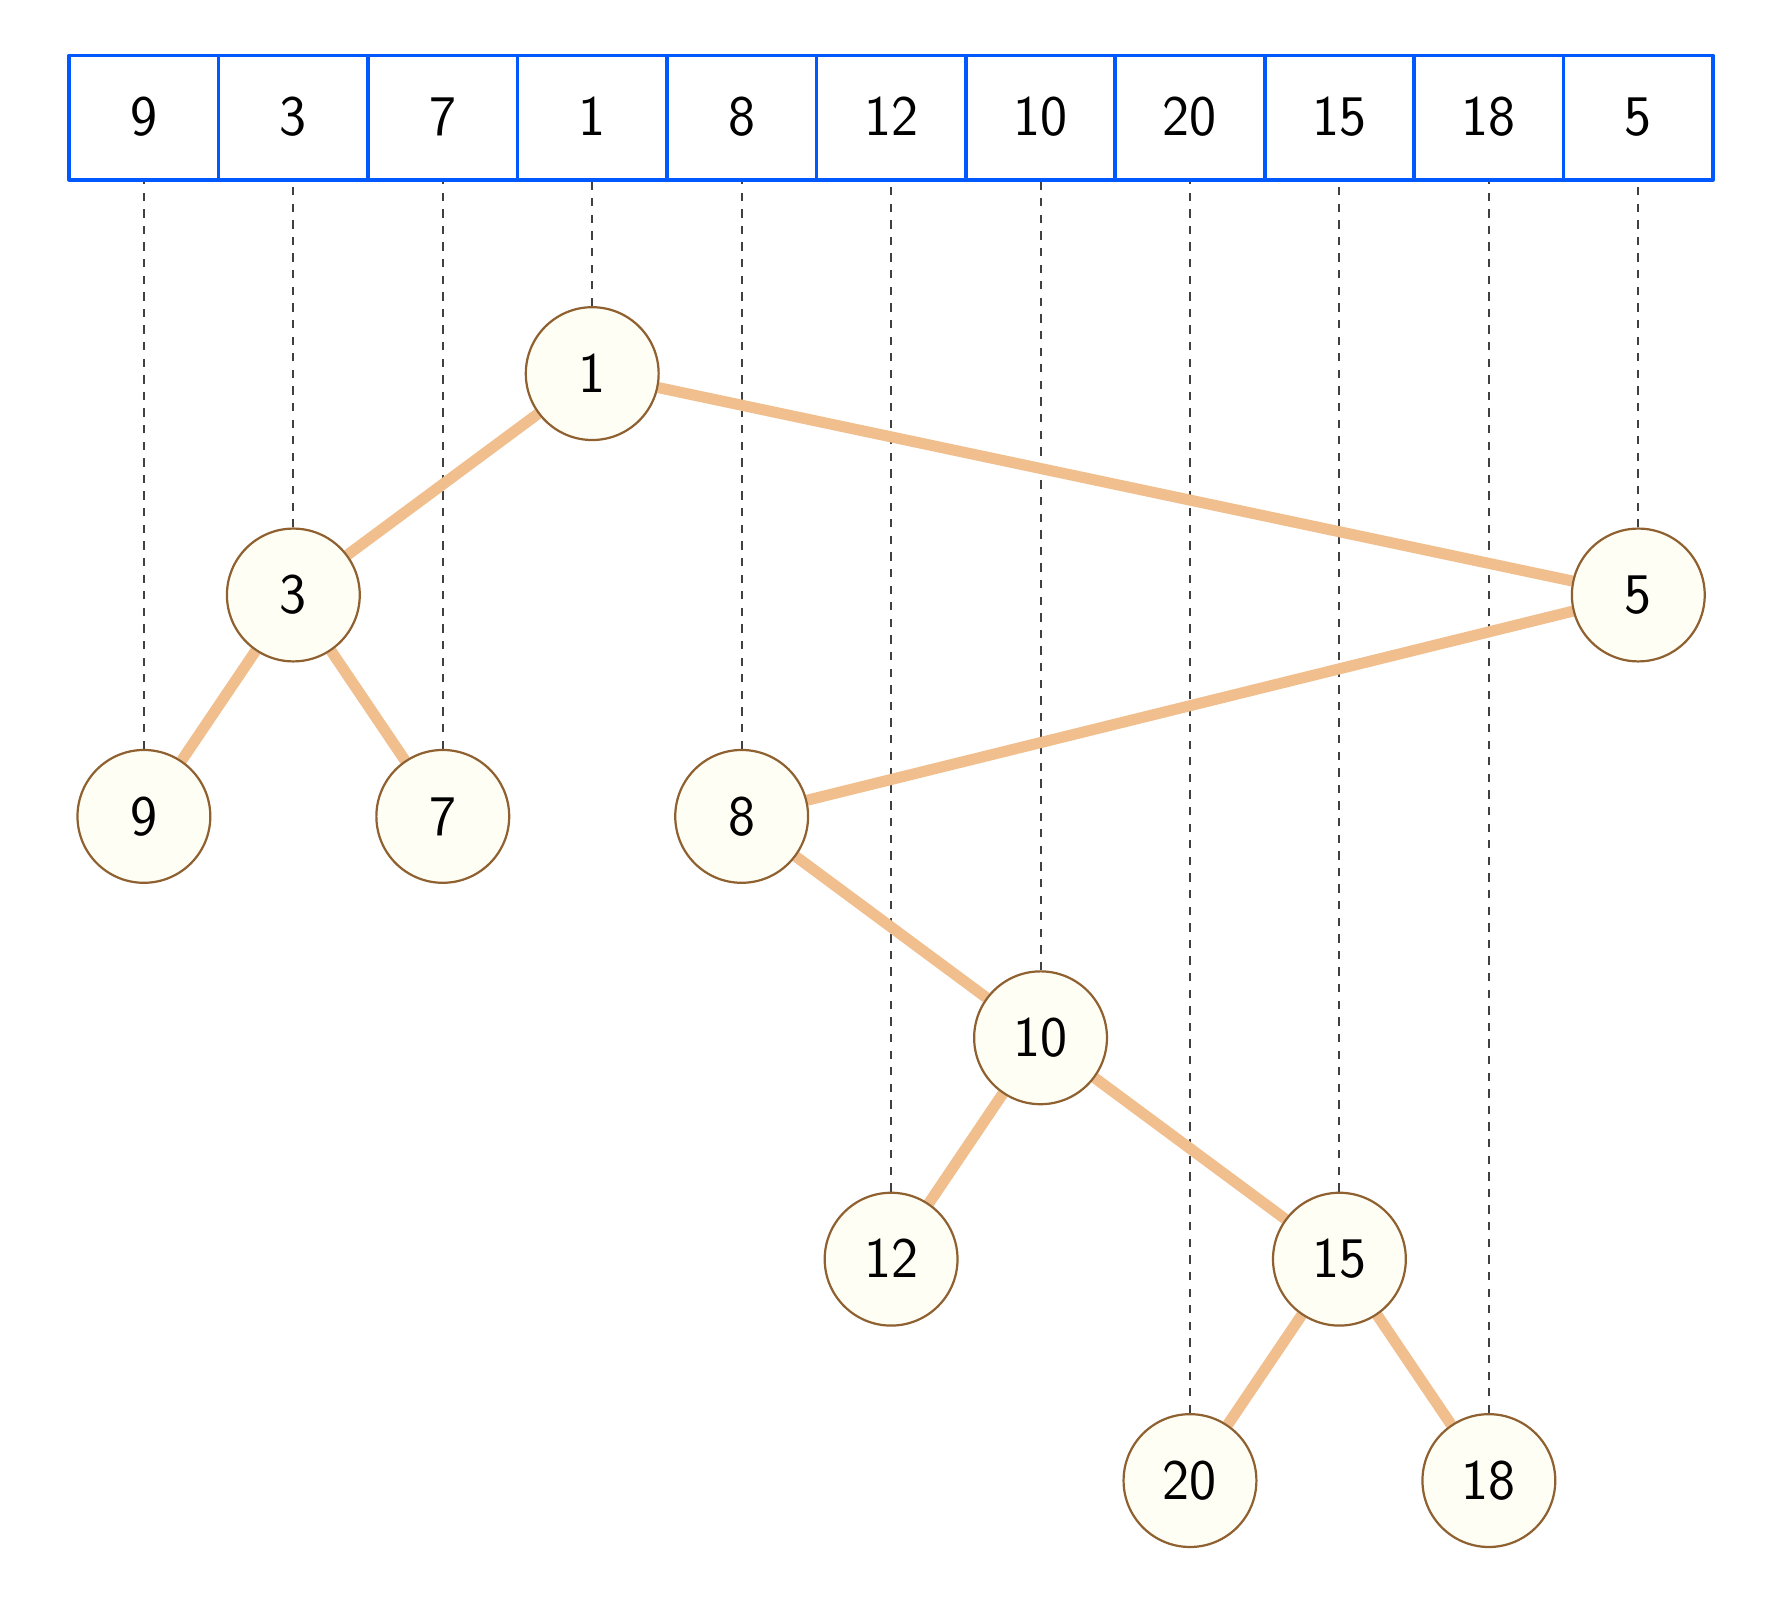
\begin{tikzpicture}[x=1pt,y=-1pt,>=Stealth,line cap=round,line join=round]
\path[use as bounding box] (0,0) rectangle (620,565);
\begin{scope}[on background layer]

\end{scope}
\node[circle,draw=brown!75!black,fill=yellow!4,text=black,minimum size=48pt,inner sep=0pt,line width=0.8pt,font=\sffamily\fontsize{22}{26.4}\selectfont] (n1) at (204,125) {1};
\node[circle,draw=brown!75!black,fill=yellow!4,text=black,minimum size=48pt,inner sep=0pt,line width=0.8pt,font=\sffamily\fontsize{22}{26.4}\selectfont] (n3) at (96,205) {3};
\node[circle,draw=brown!75!black,fill=yellow!4,text=black,minimum size=48pt,inner sep=0pt,line width=0.8pt,font=\sffamily\fontsize{22}{26.4}\selectfont] (n5) at (582,205) {5};
\node[circle,draw=brown!75!black,fill=yellow!4,text=black,minimum size=48pt,inner sep=0pt,line width=0.8pt,font=\sffamily\fontsize{22}{26.4}\selectfont] (n9) at (42,285) {9};
\node[circle,draw=brown!75!black,fill=yellow!4,text=black,minimum size=48pt,inner sep=0pt,line width=0.8pt,font=\sffamily\fontsize{22}{26.4}\selectfont] (n7) at (150,285) {7};
\node[circle,draw=brown!75!black,fill=yellow!4,text=black,minimum size=48pt,inner sep=0pt,line width=0.8pt,font=\sffamily\fontsize{22}{26.4}\selectfont] (n8) at (258,285) {8};
\node[circle,draw=brown!75!black,fill=yellow!4,text=black,minimum size=48pt,inner sep=0pt,line width=0.8pt,font=\sffamily\fontsize{22}{26.4}\selectfont] (n10) at (366,365) {10};
\node[circle,draw=brown!75!black,fill=yellow!4,text=black,minimum size=48pt,inner sep=0pt,line width=0.8pt,font=\sffamily\fontsize{22}{26.4}\selectfont] (n12) at (312,445) {12};
\node[circle,draw=brown!75!black,fill=yellow!4,text=black,minimum size=48pt,inner sep=0pt,line width=0.8pt,font=\sffamily\fontsize{22}{26.4}\selectfont] (n15) at (474,445) {15};
\node[circle,draw=brown!75!black,fill=yellow!4,text=black,minimum size=48pt,inner sep=0pt,line width=0.8pt,font=\sffamily\fontsize{22}{26.4}\selectfont] (n20) at (420,525) {20};
\node[circle,draw=brown!75!black,fill=yellow!4,text=black,minimum size=48pt,inner sep=0pt,line width=0.8pt,font=\sffamily\fontsize{22}{26.4}\selectfont] (n18) at (528,525) {18};
\begin{scope}[on background layer]
% Connect each array entry to its corresponding tree node.
\foreach \value in {9,3,7,1,8,12,10,20,15,18,5} {
  \draw[draw=black!75,dashed,line width=0.7pt]
    (n\value.north) -- (n\value.north |- 0,55);
}
\draw[draw=brown!45!orange!50,line width=4pt] (n1) -- (n3);
\draw[draw=brown!45!orange!50,line width=4pt] (n1) -- (n5);
\draw[draw=brown!45!orange!50,line width=4pt] (n3) -- (n9);
\draw[draw=brown!45!orange!50,line width=4pt] (n3) -- (n7);
\draw[draw=brown!45!orange!50,line width=4pt] (n5) -- (n8);
\draw[draw=brown!45!orange!50,line width=4pt] (n8) -- (n10);
\draw[draw=brown!45!orange!50,line width=4pt] (n10) -- (n12);
\draw[draw=brown!45!orange!50,line width=4pt] (n10) -- (n15);
\draw[draw=brown!45!orange!50,line width=4pt] (n15) -- (n20);
\draw[draw=brown!45!orange!50,line width=4pt] (n15) -- (n18);
\end{scope}
\draw[draw=blue!65!cyan,fill=white,line width=1.3pt] (15,10) rectangle (69,55);
\node[anchor=center,text=black,font=\sffamily\fontsize{22}{26.4}\selectfont] at (42,32) {9};
\draw[draw=blue!65!cyan,fill=white,line width=1.3pt] (69,10) rectangle (123,55);
\node[anchor=center,text=black,font=\sffamily\fontsize{22}{26.4}\selectfont] at (96,32) {3};
\draw[draw=blue!65!cyan,fill=white,line width=1.3pt] (123,10) rectangle (177,55);
\node[anchor=center,text=black,font=\sffamily\fontsize{22}{26.4}\selectfont] at (150,32) {7};
\draw[draw=blue!65!cyan,fill=white,line width=1.3pt] (177,10) rectangle (231,55);
\node[anchor=center,text=black,font=\sffamily\fontsize{22}{26.4}\selectfont] at (204,32) {1};
\draw[draw=blue!65!cyan,fill=white,line width=1.3pt] (231,10) rectangle (285,55);
\node[anchor=center,text=black,font=\sffamily\fontsize{22}{26.4}\selectfont] at (258,32) {8};
\draw[draw=blue!65!cyan,fill=white,line width=1.3pt] (285,10) rectangle (339,55);
\node[anchor=center,text=black,font=\sffamily\fontsize{22}{26.4}\selectfont] at (312,32) {12};
\draw[draw=blue!65!cyan,fill=white,line width=1.3pt] (339,10) rectangle (393,55);
\node[anchor=center,text=black,font=\sffamily\fontsize{22}{26.4}\selectfont] at (366,32) {10};
\draw[draw=blue!65!cyan,fill=white,line width=1.3pt] (393,10) rectangle (447,55);
\node[anchor=center,text=black,font=\sffamily\fontsize{22}{26.4}\selectfont] at (420,32) {20};
\draw[draw=blue!65!cyan,fill=white,line width=1.3pt] (447,10) rectangle (501,55);
\node[anchor=center,text=black,font=\sffamily\fontsize{22}{26.4}\selectfont] at (474,32) {15};
\draw[draw=blue!65!cyan,fill=white,line width=1.3pt] (501,10) rectangle (555,55);
\node[anchor=center,text=black,font=\sffamily\fontsize{22}{26.4}\selectfont] at (528,32) {18};
\draw[draw=blue!65!cyan,fill=white,line width=1.3pt] (555,10) rectangle (609,55);
\node[anchor=center,text=black,font=\sffamily\fontsize{22}{26.4}\selectfont] at (582,32) {5};
\end{tikzpicture}
\end{document}
